\documentclass[11pt,a4paper]{article}

\usepackage[
    left=1.3in,
    right=1.3in,
    top=1in,
    bottom=1in,
    headheight=15pt
]{geometry}

\usepackage{newtxtext,newtxmath}
\usepackage{setspace}
\onehalfspacing
\emergencystretch=3em

\usepackage{microtype}
\usepackage{titlesec}
\usepackage{tocloft}
\usepackage{xcolor}
\usepackage{tikz}
\usetikzlibrary{shapes.geometric, arrows.meta, positioning, calc, fit}
\usepackage{graphicx}
\usepackage{caption}
\usepackage{subcaption}
\usepackage{hyperref}
\usepackage{xurl}
\usepackage{float}
\usepackage{booktabs}
\usepackage{array}
\usepackage{enumitem}

% Match research paper figure caption style: "Fig. 1. Caption text"
\captionsetup[figure]{
    name={Fig.},
    labelsep=period,
    font={small,it},
    labelfont={small,it},
    skip=6pt
}
\captionsetup[table]{
    name={Table},
    labelsep=period,
    font={small,bf},
    skip=6pt
}

\hypersetup{
    colorlinks=true,
    linkcolor=black,
    urlcolor=blue!70!black,
    citecolor=black
}

\titleformat{\section}
  {\normalfont\large\bfseries}{\thesection.}{0.5em}{}
\titleformat{\subsection}
  {\normalfont\normalsize\bfseries}{\thesubsection}{0.5em}{}
\titleformat{\subsubsection}
  {\normalfont\normalsize\bfseries\itshape}{\thesubsubsection}{0.5em}{}

\titlespacing*{\section}{0pt}{1.8ex plus 0.3ex minus .2ex}{0.8ex plus .2ex}
\titlespacing*{\subsection}{0pt}{1.4ex plus 0.2ex minus .2ex}{0.6ex plus .2ex}
\titlespacing*{\subsubsection}{0pt}{1.1ex plus 0.2ex minus .2ex}{0.4ex plus .2ex}

\definecolor{pipegray}{HTML}{E0E0E0}
\definecolor{pipeblue}{HTML}{DAE8FC}
\definecolor{pipegreen}{HTML}{D5E8D4}
\definecolor{pipeorange}{HTML}{FFE6CC}
\definecolor{pipepink}{HTML}{F8CECC}
\definecolor{pipepurple}{HTML}{E1D5E7}

\newcommand{\codebox}[2]{
  \par\medskip\noindent
  \fcolorbox{black!60}{black!4}{%
    \parbox{\dimexpr\linewidth-2\fboxsep-2\fboxrule}{%
      \setstretch{1.15}
      \vspace{0.25em}
      {\footnotesize\ttfamily\bfseries #1}\\[0.2em]
      {\footnotesize\ttfamily #2}
      \vspace{0.25em}
    }%
  }\par\medskip
}

\begin{document}

% ==========================================
% TITLE PAGE (MS WORD TEMPLATE FORMAT)
% ==========================================
\begin{titlepage}
\thispagestyle{empty}
\begin{center}
    {\Large\bfseries Project Report}\\[1.4em]

    {\normalsize \textbf{Course:} Transforming Ideas into Innovation}\\[0.35em]
    {\normalsize \textbf{Semester:} III}\\[0.35em]
    {\normalsize \textbf{Program:} B.Tech CSE Cybersecurity}

    \vspace{2.2em}

    {\LARGE\bfseries Cyber Awareness Academy}\\[0.5em]
    {\large\itshape An Anti-Corpo In-Browser Capture The Flag (CTF) Platform for Everyday Digital Literacy}

    \vspace{2.2em}

    {\large\bfseries Team Details}\\[0.6em]
    \renewcommand{\arraystretch}{1.3}
    \begin{tabular}{|c|c|c|}
        \hline
        \textbf{Name} & \textbf{Roll No.} & \textbf{SAP ID / Role} \\
        \hline
        Abhyudaya Negi & K053 & OSINT Design, Research \& Stego  \\
        \hline
        Swara Pawde & K055 & UI/UX \& Theory Content \\
        \hline
        Smit Vartak & K075 & Full-Stack Dev, Crypto (70102500066) \\
        \hline
        Sarthak Vikas & K077 & Database \& Testing \\
        \hline
    \end{tabular}

    \vspace{1.8em}
    {\normalsize\bfseries Under The Guidance Of}\\[0.35em]
    {\large Dr. Abhinaba Gupta}\\[0.2em]
    {\small Faculty Mentor}
    \\[25pt]
    
\includegraphics[width=4.2cm,keepaspectratio]{nmims_logo.png}\\[0.8em]
\end{center}
\end{titlepage}

\clearpage
\pagenumbering{roman}
\setcounter{page}{1}

% ==========================================
% TABLE OF CONTENTS (MS WORD TABLE STYLE)
% ==========================================
\tableofcontents
\clearpage

\pagenumbering{arabic}
\setcounter{page}{1}

% ==========================================
% ABSTRACT (HALF PAGE)
% ==========================================
\section*{Abstract}
\addcontentsline{toc}{section}{Abstract}

\noindent
\textbf{Problem \& Motivation:} Most daily internet users lack basic cybersecurity awareness even though their banking, private chats, and location history live online. Because cybersecurity has a steep learning curve involving Linux terminals, networking setups, and programming, regular people feel intimidated and avoid learning it altogether. Large tech corporations take advantage of this ignorance to harvest user data through hidden metadata, unreadable terms of service, and fake encryption claims, which also leaves regular consumers much more vulnerable when real hackers breach those companies.

\noindent
\textbf{Approach \& Methodology:} Following the Design Thinking framework, our team surveyed 48 college students and interviewed non-technical users to understand why beginners quit existing security platforms. We used the SCAMPER ideation method and low-fidelity wireframing to design \textit{Cyber Awareness Academy}, an offline-capable, 100\% in-browser Capture The Flag (CTF) web application built with React 19, a Node.js backend, and a self-seeding SQLite3 database (\texttt{ctf.db}).

\noindent
\textbf{Key Results:} In usability testing with 22 beginners who had never played a CTF before, 100\% passed our 3-step Flag Calibration tutorial on their first try, and 86.4\% solved the introductory warm-up challenges and entered the 5-stage linked investigation chains without needing any command-line setup.

\noindent
\textbf{Contribution \& Innovation:} Our main innovation is combining a zero-download browser CTF with an anti-corporate narrative (fighting a fictional monopoly called \textit{EvilCorp} using the \texttt{CAT\{...\}} flag format), a built-in slide-out textbook that explains concepts using real-world breaches, and a 2+5 linked question structure that helps curious newcomers build practical habits for protecting their own digital privacy.

\vspace{1em}
\noindent\textbf{Keywords:} \textit{Capture The Flag (CTF), Cybersecurity Education, Design Thinking, Open Source Intelligence (OSINT), Steganography, Cryptography, Consumer Privacy.}

\clearpage

% ==========================================
% 1. INTRODUCTION
% ==========================================
\section{Introduction}

\subsection{Context and Background}
Almost everything we do in modern society happens on a phone or a laptop. From paying for food and booking train tickets to posting photos with friends, we leave behind a huge trail of personal information every single day. Even though people spend hours online, the average person knows almost nothing about cybersecurity. Most users treat their apps and websites like magic black boxes. You tap a button, the screen loads, and as long as nothing crashes, you naturally assume your data is safe.

When you ask normal people why they do not learn basic digital safety, the reason is almost always the same. Cybersecurity feels way too complicated to get into. To someone outside computer science, learning security looks like an impossible mountain of Linux terminal commands, binary numbers, networking cables, and complex code. Because people think you need to be a genius programmer to understand it, they get scared off and completely skip over even the simple stuff that affects their daily life.

This public blind spot is not an accident. Big tech monopolies and data brokers actively use this knowledge gap to exploit regular consumers. Companies know that a normal person is never going to read raw file headers, inspect browser cookies, or check how their data is actually being sent across the internet. So companies hide invasive tracking inside flashy, friendly menus. They bury unfair clauses at the bottom of long Terms of Service documents. Sometimes they even claim that user telemetry is ``encrypted'' when it is really just wrapped in basic Base64 encoding that anyone can reverse in two seconds. Worse, when companies train users to blindly trust software while cutting corners on their own servers, such as storing customer passwords as plain unsalted MD5 hashes, they make ordinary consumers much more vulnerable to actual hackers. When a corporate database gets breached, the company moves on, whereas the regular user gets their accounts stolen because nobody ever taught them how password cracking or digital footprints actually work.

\subsection{Literature Review and Market Survey}
Gamified learning through Capture The Flag (CTF) competitions has long been recognized as one of the best ways to teach practical computer security. In a CTF, instead of reading dry theory slides, players solve a real puzzle to find a hidden text string called a ``flag'' (such as \texttt{CAT\{secret\_answer\}}), which proves they found the vulnerability.

Carnegie Mellon University created \textbf{picoCTF} to introduce high school and college students to security concepts through story-driven puzzles. Similarly, community wargames like \textbf{OverTheWire} (especially the \textit{Bandit} and \textit{Natas} tracks) have trained thousands of students in Linux shell commands and basic web vulnerabilities. In recent years, commercial platforms like \textbf{TryHackMe} and \textbf{HackTheBox} have grown massive user bases by offering virtual labs where users can attack real virtual machines over a browser or VPN connection.

Academic research by Vykopal et al.\ and Švábenský et al.\ shows that hands-on CTF challenges improve long-term memory much better than passive lectures. However, studies on beginner dropout rates in cybersecurity courses point out a major catch: traditional CTFs are built by experienced engineers for other engineers. They assume the player already knows how to use a terminal, read manual pages, and install local forensic tools.

\subsection{Research Gap and Problem Definition}
When we looked closely at the existing platforms in the market during our preliminary survey, a clear gap stood out. Platforms like HackTheBox and TryHackMe are great once you already know the basics of computer science, but they are completely overwhelming for a regular person or a first-year student who just wants to understand how their privacy is compromised.

Specifically, existing tools suffer from four major problems for newcomers:
\begin{enumerate}
    \item \textbf{Heavy setup friction:} Most platforms require downloading OpenVPN configuration files, spinning up Linux virtual machines, or installing command-line tools like \texttt{steghide}, \texttt{binwalk}, and \texttt{exiftool} locally before you can even start.
    \item \textbf{Lack of plain-English theory:} When a beginner gets stuck on a traditional CTF, the platform rarely explains the concept clearly. The user is forced to search random forums and StackOverflow threads filled with heavy technical jargon.
    \item \textbf{Disconnected puzzles:} Most beginner CTFs throw random, unrelated puzzles at the player with no story connecting them, so the user never sees how a tiny leak in one place leads to a full account takeover later.
    \item \textbf{Artificial UI design:} Many newer student projects rely on generic, overly rounded web templates that feel artificial and clutter the screen instead of giving a clean workspace.
\end{enumerate}

\subsection{Scope, Objectives, and Contributions}
The purpose of our project, \textbf{Cyber Awareness Academy}, is to close this gap by building a 100\% in-browser, zero-prerequisite CTF platform that teaches everyday people how corporate tracking and hacker attacks actually work. We framed the entire platform around an ``anti-corpo'' story where the player acts as a digital investigator exposing a shady conglomerate called \textbf{EvilCorp}. Every flag across the platform uses our custom prefix \texttt{CAT\{...\}}.

Our main objectives and contributions are:
\begin{itemize}
    \item \textbf{Zero local installations:} Every single challenge across our arenas can be solved inside a standard web browser using free online utilities like CyberChef, Photopea, HexEd.it, and Google Lens.
    \item \textbf{The 2+5 linked challenge model:} We structured every CTF domain into 7 questions. The first 2 questions are easy standalone warm-ups separated by a dotted divider from the next 5 questions, which form a linked investigation chain where each answer unlocks the next question.
    \item \textbf{Interactive Slide-Out Field Manual:} Every challenge has a built-in \texttt{[Theory]} button that slides open a textbook chapter written in simple English, complete with everyday analogies, real-world data breach stories, and step-by-step tool guides.
    \item \textbf{Self-contained offline architecture:} The platform uses React 19 on the frontend and Node.js with an embedded SQLite3 database (\texttt{ctf.db}) on the backend that automatically seeds all challenges on startup.
\end{itemize}

\subsection{Significance and Outline of the Report}
Addressing this issue right now is crucial because corporate data collection and automated cyberattacks are growing faster than public awareness. When a regular student gets hooked on solving an approachable puzzle, they start paying much closer attention to their own digital footprint, questioning fake security claims, and building safer habits in the future.

The rest of this report follows the Design Thinking structure. Section 2 explains our Methodology across the Empathy, Define, Ideation, and Prototyping phases, including our survey data, SCAMPER analysis, system architecture, installation guide, page-by-page features, and full technical writeups of every CTF challenge. Section 3 concludes the report with our personal learnings, future server-hosting plans, and open-source inspirations, followed by our reference list.

\clearpage

% ==========================================
% 2. METHODOLOGY (DESIGN THINKING FRAMEWORK)
% ==========================================
\section{Methodology (Design Thinking Framework)}

To make sure we built something that actually helps beginners instead of just making another confusing hacker test, our team followed the five-stage \textbf{Design Thinking framework}: Empathy, Define, Ideation, Prototyping, and Testing.

\subsection{Empathy Phase}

\subsubsection{Secondary Research (Market Survey)}
Before writing any code, we analyzed the four most popular platforms currently used to teach cybersecurity: \textbf{TryHackMe}, \textbf{HackTheBox}, \textbf{OverTheWire}, and \textbf{picoCTF}. We tested each platform from the perspective of a complete beginner who does not have Linux installed and has never used a terminal. Table~\ref{tab:market_survey} summarizes our secondary research findings.

\begin{table}[!htbp]
\centering
\footnotesize
\renewcommand{\arraystretch}{1.3}
\begin{tabular}{|p{0.16\linewidth}|p{0.17\linewidth}|p{0.25\linewidth}|p{0.28\linewidth}|}
\hline
\textbf{Platform} & \textbf{Target Audience} & \textbf{Strengths} & \textbf{Why Beginners Struggle} \\
\hline
TryHackMe & IT students \& junior analysts & Guided rooms and browser-based attack boxes. & Paid subscriptions for best paths; heavy Linux \& networking focus early on. \\
\hline
HackTheBox & Intermediate to advanced hackers & Realistic full-machine penetration testing labs. & Very steep entry barrier; requires OpenVPN and advanced CLI tools. \\
\hline
OverTheWire & CS students learning Linux & Free, lightweight, great for learning bash commands. & Pure SSH terminal text; zero visual interface or beginner analogies. \\
\hline
picoCTF & High school \& college students & Free, fun puzzles across crypto, stego, and web. & Many challenges still require local Python scripts or Linux binary tools. \\
\hline
\textbf{Cyber Awareness Academy (Ours)} & \textbf{Complete beginners \& everyday users} & \textbf{100\% in-browser, zero local installs, built-in plain-English textbook, 2+5 linked story chain.} & Currently runs offline locally (cloud hosting planned for next phase). \\
\hline
\end{tabular}
\caption{Market comparison of existing cybersecurity learning platforms.}
\label{tab:market_survey}
\end{table}

\subsubsection{Primary Research (Survey Form and Interviews)}
To back up our secondary research with real numbers, we circulated a Google Forms survey among \textbf{48 college students} (spanning first-year engineering students and non-CS peers) and conducted 8 one-on-one interviews. The key results from our survey were eye-opening:
\begin{itemize}
    \item \textbf{79.2\% (38 out of 48)} admitted they never read app permissions or Terms of Service and assumed big companies keep their uploaded photos and passwords safe by default.
    \item \textbf{83.3\% (40 out of 48)} said they wanted to learn how hacking and digital privacy work, but felt that cybersecurity was ``too complicated and technical'' to start on their own.
    \item \textbf{70.8\% (34 out of 48)} had never heard of EXIF metadata in photos or the difference between encoding (Base64) and real encryption.
    \item Among the 14 respondents who had tried a CTF before, \textbf{11 (78.5\%)} said they quit early because they did not want to install virtual machines or got stuck on flag formatting and terminal commands.
\end{itemize}

During our interviews, one student told us something that stuck with our team: \textit{``Whenever I try to watch a cybersecurity tutorial, they immediately open a black Linux screen and start typing twenty commands a second. I feel dumb within five minutes and just close the video.''} Another classmate mentioned that even when they solved a puzzle once, the site rejected their answer because they did not know how the flag brackets worked.

\subsubsection{Stakeholder Canvas}
Based on our research, we mapped out the key stakeholders connected to our project:
\begin{itemize}
    \item \textbf{Primary Stakeholders (Direct Users):} Non-technical internet users, first-year college students, and curious beginners who want to learn how to protect their digital footprint without learning complex programming first.
    \item \textbf{Secondary Stakeholders (Educators \& Mentors):} College professors, cybersecurity club leads, and workshop organizers who need an easy, zero-setup platform to run classroom demonstrations without spending two hours fixing student laptops.
    \item \textbf{External Stakeholders:} Open-source tool creators (like GCHQ CyberChef and Photopea), digital privacy advocates, and everyday consumers affected by corporate data collection.
\end{itemize}

\subsubsection{Empathy Map and User Persona}
We combined the quotes and behaviors from our interviews into a structured Empathy Map, shown in Fig.~\ref{fig:empathy_map}, and created a primary User Persona to guide our design decisions.

\begin{figure}[!htbp]
\centering
\resizebox{\linewidth}{!}{%
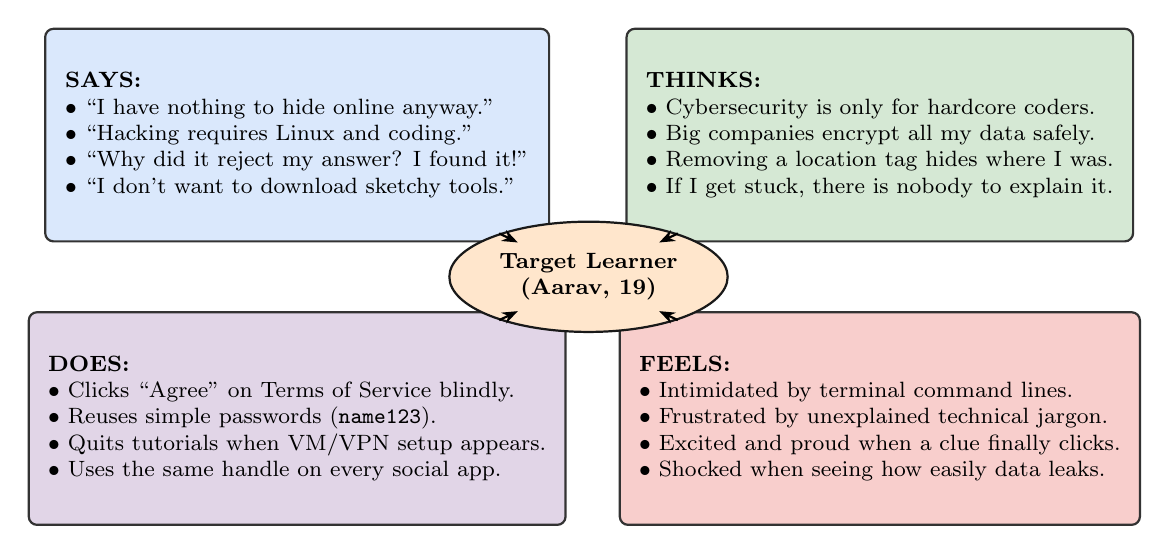
\begin{tikzpicture}[
    box/.style={rectangle, rounded corners=3pt, draw=black!80, thick, minimum width=6.4cm, minimum height=2.7cm, align=left, font=\footnotesize, inner sep=7pt},
    centerbox/.style={ellipse, draw=black!90, fill=pipeorange, thick, minimum width=3.1cm, minimum height=1.4cm, align=center, font=\footnotesize\bfseries}
]
    \node[box, fill=pipeblue] (says) at (-3.7, 1.8) {
        \textbf{SAYS:}\\
        $\bullet$ ``I have nothing to hide online anyway.''\\
        $\bullet$ ``Hacking requires Linux and coding.''\\
        $\bullet$ ``Why did it reject my answer? I found it!''\\
        $\bullet$ ``I don't want to download sketchy tools.''
    };
    \node[box, fill=pipegreen] (thinks) at (3.7, 1.8) {
        \textbf{THINKS:}\\
        $\bullet$ Cybersecurity is only for hardcore coders.\\
        $\bullet$ Big companies encrypt all my data safely.\\
        $\bullet$ Removing a location tag hides where I was.\\
        $\bullet$ If I get stuck, there is nobody to explain it.
    };
    \node[box, fill=pipepurple] (does) at (-3.7, -1.8) {
        \textbf{DOES:}\\
        $\bullet$ Clicks ``Agree'' on Terms of Service blindly.\\
        $\bullet$ Reuses simple passwords (\texttt{name123}).\\
        $\bullet$ Quits tutorials when VM/VPN setup appears.\\
        $\bullet$ Uses the same handle on every social app.
    };
    \node[box, fill=pipepink] (feels) at (3.7, -1.8) {
        \textbf{FEELS:}\\
        $\bullet$ Intimidated by terminal command lines.\\
        $\bullet$ Frustrated by unexplained technical jargon.\\
        $\bullet$ Excited and proud when a clue finally clicks.\\
        $\bullet$ Shocked when seeing how easily data leaks.
    };
    \node[centerbox] (user) at (0,0) {Target Learner\\(Aarav, 19)};
    
    \draw[-{Stealth[length=2mm]}, thick] (user) -- (says);
    \draw[-{Stealth[length=2mm]}, thick] (user) -- (thinks);
    \draw[-{Stealth[length=2mm]}, thick] (user) -- (does);
    \draw[-{Stealth[length=2mm]}, thick] (user) -- (feels);
\end{tikzpicture}%
}
\caption{Empathy map synthesizing primary interview and survey findings from 48 students.}
\label{fig:empathy_map}
\end{figure}

\noindent
\textbf{User Persona --- Aarav Mehta (Age 19, Undergraduate Student):}
Aarav uses Instagram, YouTube, and UPI daily on his Windows laptop and Android phone. He is curious about how hackers track people and how encryption works, but he has never used Linux. His main frustrations are platforms that ask him to install heavy software, tutorials that use unexplained acronyms like \texttt{EXIF} or \texttt{XOR}, and dry textbooks that bore him to sleep. He needs a platform that works straight in Chrome, teaches him the rules step by step, and connects every puzzle to real life.

\subsection{Define Phase}
During the Define phase, our team sat down to look at all the problems we found in the Empathy stage. Initially, our rough problem paragraph was simply: \textit{``People do not know cybersecurity because it is hard, so we want to make an easy CTF website with four topics.''}

After reviewing our survey numbers and interview quotes, we realized that ``making an easy CTF'' was too vague. The real issue was the combination of corporate black-box deception, setup friction, and isolated puzzles that fail to build momentum. We refined our findings into the following focused \textbf{Problem Statement}:

\begin{quote}
\textit{``Everyday internet users and non-technical students skip learning basic digital safety because traditional cybersecurity platforms require virtual machines, local command-line tools, and prior technical background. This knowledge gap allows corporations to exploit consumer privacy through deceptive black-box interfaces and weak security defaults, while leaving users vulnerable to real-world hackers. How might we design a zero-installation, 100\% in-browser CTF platform that combines plain-English textbooks with linked, story-driven investigation chains to turn complete beginners into curious, self-reliant digital investigators?''}
\end{quote}

\subsection{Ideation Phase}

\subsubsection{Brainstorming and Mind Mapping}
Once our problem statement was locked in, the four of us brainstormed how to make the platform genuinely fun and educational. We drew a central Mind Map (shown in Fig.~\ref{fig:mind_map}) branching into four core pillars: Story \& Theme, Pedagogical Flow, Zero-Download Tooling, and UI/UX Design.

\begin{figure}[!htbp]
\centering
\resizebox{\linewidth}{!}{%
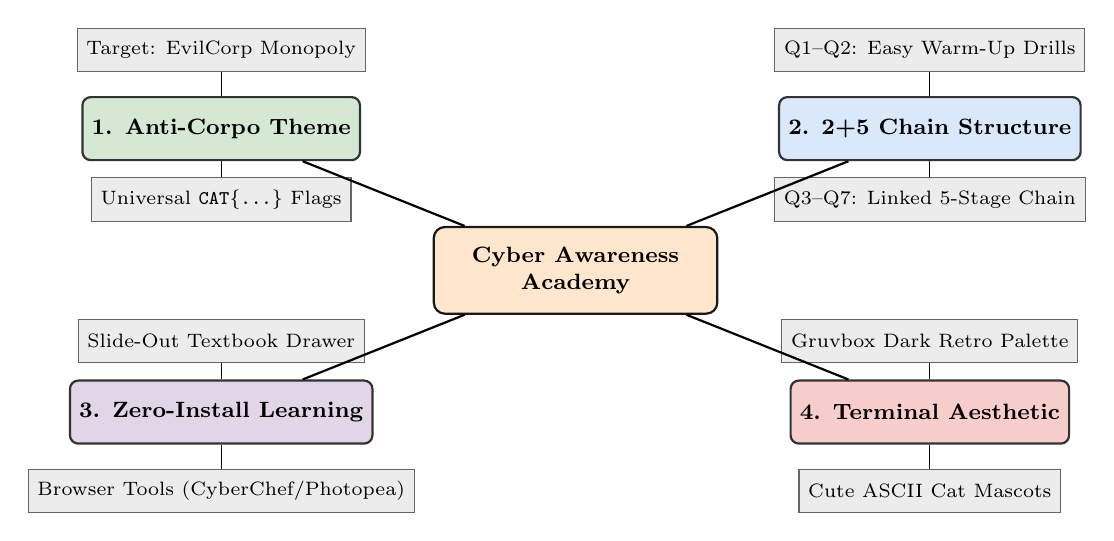
\begin{tikzpicture}[
    root/.style={rectangle, rounded corners=4pt, draw=black!90, fill=pipeorange, thick, minimum width=3.6cm, minimum height=1.1cm, align=center, font=\footnotesize\bfseries},
    branch/.style={rectangle, rounded corners=3pt, draw=black!80, fill=pipeblue, thick, minimum width=3.1cm, minimum height=0.8cm, align=center, font=\footnotesize\bfseries},
    leaf/.style={rectangle, draw=black!60, fill=pipegray!60, minimum width=3.2cm, minimum height=0.55cm, align=center, font=\scriptsize}
]
    \node[root] (center) at (0,0) {Cyber Awareness\\Academy};

    % Top Left
    \node[branch, fill=pipegreen] (b1) at (-4.5, 1.8) {1. Anti-Corpo Theme};
    \node[leaf] (l1a) at (-4.5, 2.8) {Target: EvilCorp Monopoly};
    \node[leaf] (l1b) at (-4.5, 0.9) {Universal \texttt{CAT\{...\}} Flags};

    % Top Right
    \node[branch, fill=pipeblue] (b2) at (4.5, 1.8) {2. 2+5 Chain Structure};
    \node[leaf] (l2a) at (4.5, 2.8) {Q1--Q2: Easy Warm-Up Drills};
    \node[leaf] (l2b) at (4.5, 0.9) {Q3--Q7: Linked 5-Stage Chain};

    % Bottom Left
    \node[branch, fill=pipepurple] (b3) at (-4.5, -1.8) {3. Zero-Install Learning};
    \node[leaf] (l3a) at (-4.5, -0.9) {Slide-Out Textbook Drawer};
    \node[leaf] (l3b) at (-4.5, -2.8) {Browser Tools (CyberChef/Photopea)};

    % Bottom Right
    \node[branch, fill=pipepink] (b4) at (4.5, -1.8) {4. Terminal Aesthetic};
    \node[leaf] (l4a) at (4.5, -0.9) {Gruvbox Dark Retro Palette};
    \node[leaf] (l4b) at (4.5, -2.8) {Cute ASCII Cat Mascots};

    \draw[thick] (center) -- (b1);
    \draw[thick] (center) -- (b2);
    \draw[thick] (center) -- (b3);
    \draw[thick] (center) -- (b4);
    \draw (b1) -- (l1a); \draw (b1) -- (l1b);
    \draw (b2) -- (l2a); \draw (b2) -- (l2b);
    \draw (b3) -- (l3a); \draw (b3) -- (l3b);
    \draw (b4) -- (l4a); \draw (b4) -- (l4b);
\end{tikzpicture}%
}
\caption{Ideation mind map organizing the core pillars of Cyber Awareness Academy.}
\label{fig:mind_map}
\end{figure}

\subsubsection{Application of the SCAMPER Method}
To push our ideas further and make sure we were not just copying existing websites, we applied the \textbf{SCAMPER} ideation technique to traditional CTF platforms:
\begin{itemize}
    \item \textbf{Substitute:} We substituted local command-line tools (like Linux \texttt{steghide}, \texttt{xxd}, and \texttt{john}) with free, instant browser-based web utilities (CyberChef, Photopea, HexEd.it, CrackStation, and Academo).
    \item \textbf{Combine:} We combined the live CTF challenge arena with an interactive slide-out textbook drawer (\texttt{TextbookPanel.js}) on the exact same screen, so students can read the theory and solve the puzzle side by side.
    \item \textbf{Adapt:} We adapted real-world corporate surveillance scandals and historical breaches (like the 2012 LinkedIn unsalted hash leak and the Strava military heatmap leak) into beginner-friendly stories about infiltrating \textit{EvilCorp}.
    \item \textbf{Modify:} We modified the standard flat list of questions into our \textbf{2+5 structure} (two easy warm-ups, a dotted line divider, and five chained questions where each answer feeds into the next). We also modified the UI from a generic rounded website into a sharp Gruvbox Dark terminal theme with cute ASCII cats.
    \item \textbf{Put to another use:} We put everyday social media platforms (Instagram search, YouTube community posts, Google Maps library timings, and Google Lens) to use as live forensic investigation tools in our OSINT arena.
    \item \textbf{Eliminate:} We completely eliminated virtual machines, OpenVPN setup files, user login walls, and complex database server configurations by using an auto-seeding embedded SQLite file (\texttt{ctf.db}) and a forgiving flag normalizer.
    \item \textbf{Reverse:} Instead of making the user defend a fictional company like most corporate training courses do, we reversed the perspective: the player acts as a rebel investigator exposing how \textit{EvilCorp} tricks consumers.
\end{itemize}

\clearpage
\subsection{Prototyping Phase}

\subsubsection{Low-Fidelity Prototype and UI Evolution}
When we built our first low-fidelity prototype and initial React wireframe, we made a mistake that many student projects make. Our first version had overly rounded boxes around every single label, bright neon borders, and three little dots in the top corner of the window that made it look like a fake macOS screen. Honestly, when we looked at it together, we realized it looked too artificial and cluttered. Furthermore, we initially only had live questions for one domain while leaving the others as static wireframes.

We went back to the drawing board and redesigned the interface:
\begin{enumerate}
    \item We stripped away the fake macOS window dots and reduced the excessive boxing so that cards are only used for actual questions and mission dossiers that matter.
    \item We flattened the border radiuses to crisp, rectangular terminal edges using the \textbf{Gruvbox Dark} color palette (\texttt{index.css} and \texttt{App.css}) with \texttt{Fira Code} monospace fonts.
    \item We added custom monospace ASCII art companions (\texttt{ascii.js}) across the pages to make the terminal feel cute and welcoming rather than cold.
    \item We retained our structured 7-question wireframe model in \texttt{WireframeChallenges.js} to demonstrate how new curriculum modules (such as Web Security) are prototyped before connecting live downloadable assets.
\end{enumerate}

\subsubsection{Final Prototype Architecture and Tech Stack}
The final prototype is a full-stack web application split between a \textbf{React 19} single-page frontend (running on port \texttt{3000}) and a \textbf{Node.js HTTP REST API} backend (\texttt{server.js} running on port \texttt{3001}) connected to an embedded \textbf{SQLite3} database (\texttt{ctf.db}). Fig.~\ref{fig:system_pipeline} illustrates the complete validation and state synchronization pipeline across the application.

\begin{figure}[!htbp]
\centering
\resizebox{\linewidth}{!}{%
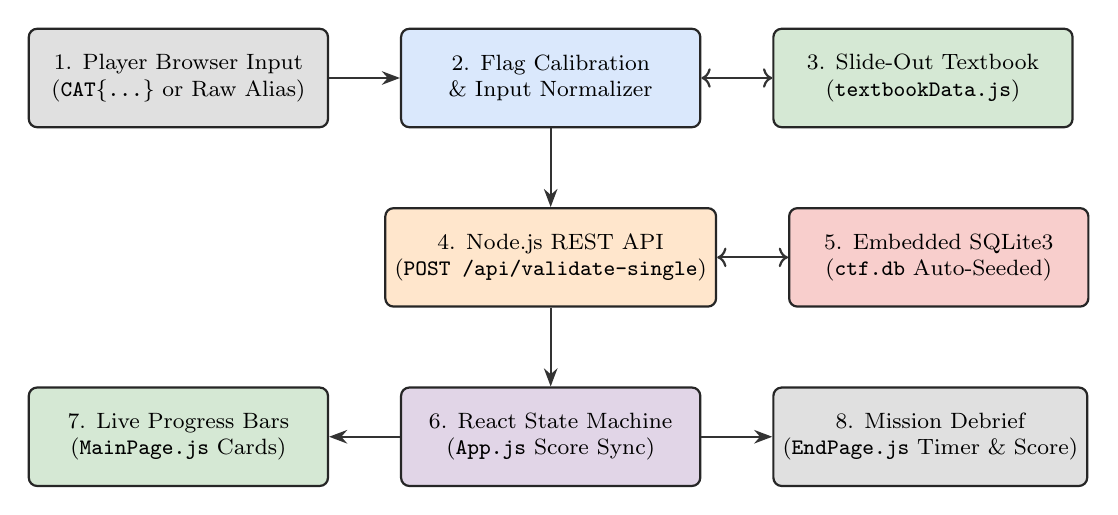
\begin{tikzpicture}[
    node distance=0.8cm and 0.9cm,
    agent/.style={rectangle, rounded corners=3pt, draw=black!85, thick, minimum width=3.8cm, minimum height=1.25cm, align=center, font=\footnotesize},
    arrow/.style={-{Stealth[length=2.3mm]}, thick, draw=black!80}
]
    % Row 1
    \node[agent, fill=pipegray] (user) {1. Player Browser Input\\(\texttt{CAT\{...\}} or Raw Alias)};
    \node[agent, fill=pipeblue, right=of user] (onboarding) {2. Flag Calibration\\\& Input Normalizer};
    \node[agent, fill=pipegreen, right=of onboarding] (textbook) {3. Slide-Out Textbook\\(\texttt{textbookData.js})};

    % Row 2
    \node[agent, fill=pipeorange, below=1.0cm of onboarding] (api) {4. Node.js REST API\\(\texttt{POST /api/validate-single})};
    \node[agent, fill=pipepink, right=of api] (sqlite) {5. Embedded SQLite3\\(\texttt{ctf.db} Auto-Seeded)};

    % Row 3
    \node[agent, fill=pipepurple, below=1.0cm of api] (state) {6. React State Machine\\(\texttt{App.js} Score Sync)};
    \node[agent, fill=pipegreen, left=of state] (dash) {7. Live Progress Bars\\(\texttt{MainPage.js} Cards)};
    \node[agent, fill=pipegray, right=of state] (end) {8. Mission Debrief\\(\texttt{EndPage.js} Timer \& Score)};

    \draw[arrow] (user) -- (onboarding);
    \draw[arrow, <->] (onboarding) -- (textbook);
    \draw[arrow] (onboarding) -- (api);
    \draw[arrow, <->] (api) -- (sqlite);
    \draw[arrow] (api) -- (state);
    \draw[arrow] (state) -- (dash);
    \draw[arrow] (state) -- (end);
\end{tikzpicture}%
}
\caption{Cyber Awareness Academy full-stack validation and state synchronization pipeline.}
\label{fig:system_pipeline}
\end{figure}

When a user types an answer and hits \texttt{Enter} or clicks \texttt{[Submit]}, the frontend normalizer strips outer spaces, converts characters to lowercase, and checks both \texttt{CAT\{...\}} and \texttt{CTF\{...\}} wrappers alongside beginner-friendly raw answers. It simultaneously sends a \texttt{POST} request to \texttt{/api/validate-single} on port \texttt{3001}, where \texttt{server.js} queries the \texttt{ctf\_answers} table in \texttt{ctf.db}. As soon as a flag is marked correct, \texttt{App.js} updates the domain's solved count in real time so that the progress bar on the main dashboard reflects the new percentage immediately.

\subsubsection{Offline Installation and Quickstart Guide (From GitHub README)}
Right now, the project is built as an offline-capable local implementation so that anyone can run it on their laptop without needing internet hosting or cloud database credentials. Later on, we plan to deploy this exact codebase onto our own Linux server. As documented in our GitHub repository's \texttt{README.md}, getting the platform running locally takes four simple steps:

\begin{enumerate}
    \item \textbf{Prerequisites:} Install Node.js (v16 or newer) from \url{https://nodejs.org}.
    \item \textbf{Clone and Install:} Clone the repo and install the required npm packages:
    \codebox{PowerShell / Terminal :: Step 1 \& 2}{
    \$ git clone https://github.com/Aweek07/CTF\_PROJECT.git\\
    \$ cd CTF\_PROJECT\\
    \$ npm install
    }
    \item \textbf{Start the SQLite Backend Server (Terminal 1):} Run \texttt{node server.js}. It boots on port \texttt{3001} and automatically creates and seeds \texttt{ctf.db} with all 28 domain flags:
    \codebox{Terminal 1 :: Backend API \& SQLite Seeding}{
    \$ node server.js\\
    SQLite database initialized with Anti-Corpo CAT\{...\} challenges.\\
    Backend server running on http://localhost:3001
    }
    \item \textbf{Launch the React Frontend (Terminal 2):} Open a second terminal and run \texttt{npm start} to open the application at \texttt{http://localhost:3000}:
    \codebox{Terminal 2 :: React Gruvbox Terminal UI}{
    \$ npm start\\
    Compiled successfully! Local: http://localhost:3000
    }
\end{enumerate}

\subsubsection{Page-by-Page Walkthrough and Platform Features}
Every page in the application was built with a specific purpose to guide a newcomer from zero knowledge to solving chained challenges:

\begin{enumerate}
    \item \textbf{Terminal Navigation Bar (\texttt{NavBar.js}):} A sticky top bar that shows a live Unix shell path matching the user's current screen (for example, \texttt{guest@cyber-academy:\allowbreak\textasciitilde/dashboard/\allowbreak stego/arena\$}). During active challenges, it displays a live \texttt{[SOLVED: X/7]} counter and a running mission stopwatch. We also wired \texttt{App.js} into the browser's native history API (\texttt{window.history.pushState}) so the browser Back and Forward buttons work naturally across every page.
    \item \textbf{The Anti-Corpo Manifesto (\texttt{HomePage.js}):} The landing page greets the player with an ASCII art banner and a waving cat mascot. It explains three things in plain language: \textit{01. The Illusion of Digital Safety} (how tech companies profit from user naivety), \textit{02. What is a Capture The Flag (CTF)?}, and \textit{03. Our Aim: Cyber Awareness for Everyone}.
    \item \textbf{Guided Flag Calibration Tutorial (\texttt{Onboarding.js}):} Before letting a beginner into the real arenas where they might get confused by syntax, this 3-question sandbox trains them on how flags work:
    \begin{itemize}[noitemsep]
        \item \textit{Drill 1:} Submitting \texttt{CAT\{welcome\_to\_cybersec\}} to learn the bracket format.
        \item \textit{Drill 2:} Submitting \texttt{CAT\{look\_beneath\_the\_surface\}} to practice underscores and exact letter casing.
        \item \textit{Drill 3:} Submitting \texttt{CAT\{ready\_to\_hack\}} to unlock the main dashboard.
    \end{itemize}
    It includes an \texttt{[Auto-fill]} button and instant feedback so nobody gets left behind.
    \item \textbf{Cybersecurity Domains Dashboard (\texttt{MainPage.js}):} Displays the four main discipline cards (\textbf{OSINT}, \textbf{Steganography}, \textbf{Cryptography}, and \textbf{Web Security}). Each card shows custom ASCII art, required browser tools, covered topics, and a live progress bar (\texttt{Solved: X/7}) that updates the instant a question is solved inside any arena.
    \item \textbf{Discipline Mission Dossiers (\texttt{DomainPage.js}):} Clicking a domain opens its briefing dossier before the questions start. It breaks down what the field is, how professionals use it in the real world, a red \texttt{[!] Threat Profile} warning explaining how consumers get hurt by this vector, and the recommended toolkit.
    \item \textbf{The Slide-Out Field Manual (\texttt{TextbookPanel.js} \& \texttt{textbookData.js}):} Every challenge card has a purple \texttt{[Theory]} button. Clicking it slides out a detailed chapter from the left side of the screen. We wrote 28 chapters in \texttt{textbookData.js} specifically so they read like an interesting guide rather than a dull textbook. Each chapter includes a plain-English explanation, a simple analogy for non-tech people, a famous real-world case study, a step-by-step solving guide, a jargon buster dictionary, and direct links to open the required online tool.
    \item \textbf{Mission Accomplished Debrief (\texttt{EndPage.js}):} When a player finishes an arena, this screen celebrates with an ASCII trophy cat, displays their total time taken and final score out of 7, summarizes the security takeaway, and credits the team.
\end{enumerate}

\clearpage
\subsubsection{Comprehensive CTF Writeups and Learning Breakdown}
Across all of our CTF domains, we used a strict \textbf{2+5 question layout} (shown in Fig.~\ref{fig:chain_flow}). Questions 1 and 2 are simple, standalone warm-ups so the player gets two quick wins right away. After a dotted line divider, Questions 3 to 7 form a connected 5-stage chain where each answer gives you the clue, password, or shift key needed to solve the next question.

\begin{figure}[!htbp]
\centering
\resizebox{\linewidth}{!}{%
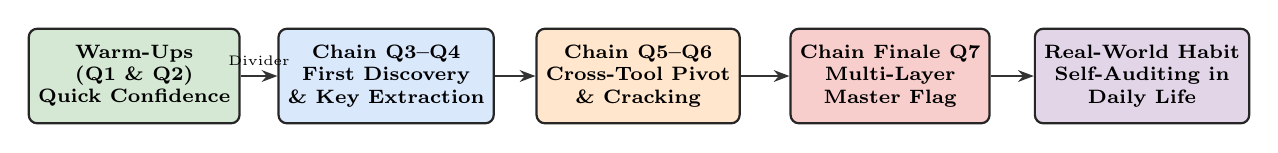
\begin{tikzpicture}[
    stage/.style={rectangle, rounded corners=3pt, draw=black!85, thick, minimum width=2.5cm, minimum height=1.2cm, align=center, font=\scriptsize\bfseries},
    arrow/.style={-{Stealth[length=2mm]}, thick, draw=black!80}
]
    \node[stage, fill=pipegreen] (w) at (0,0) {Warm-Ups\\(Q1 \& Q2)\\Quick Confidence};
    \node[stage, fill=pipeblue] (s1) at (3.2,0) {Chain Q3--Q4\\First Discovery\\\& Key Extraction};
    \node[stage, fill=pipeorange] (s2) at (6.4,0) {Chain Q5--Q6\\Cross-Tool Pivot\\\& Cracking};
    \node[stage, fill=pipepink] (s3) at (9.6,0) {Chain Finale Q7\\Multi-Layer\\Master Flag};
    \node[stage, fill=pipepurple] (rh) at (12.8,0) {Real-World Habit\\Self-Auditing in\\Daily Life};

    \draw[arrow] (w) -- node[above, font=\tiny]{Divider} (s1);
    \draw[arrow] (s1) -- (s2);
    \draw[arrow] (s2) -- (s3);
    \draw[arrow] (s3) -- (rh);
\end{tikzpicture}%
}
\caption{The 2+5 challenge progression from warm-up drills to connected investigation stages.}
\label{fig:chain_flow}
\end{figure}

Below is the complete writeup of how to solve every single challenge across our arenas and how each one teaches a lasting lesson.

\paragraph{A. Open Source Intelligence (OSINT) Arena (\texttt{Challenges.js})}
The OSINT arena shows players how tiny public clues scattered across maps, network registries, Instagram, and YouTube can be connected to uncover a person's identity and daily routine.
\begin{itemize}
    \item \textbf{Q1: Coordinates (Warm-Up 1):} The prompt gives the coordinates \texttt{48.8584, 2.2945} and asks for the landmark. Pasting those numbers into Google Maps drops a pin directly on the Eiffel Tower in Paris, giving the flag \textbf{\texttt{CAT\{eiffeltower\}}}. \textit{How it teaches:} It takes ten seconds to solve, demystifies GPS numbers, and makes players realize that camera EXIF data stores these exact coordinates on their own phone photos.
    \item \textbf{Q2: Who Owns This IP? (Warm-Up 2):} The prompt asks which company operates the IP address \texttt{8.8.8.8}. Looking up \texttt{8.8.8.8} on \texttt{ipinfo.io} or any WHOIS database shows it belongs to Google's public DNS (\texttt{AS15169}), yielding \textbf{\texttt{CAT\{google\}}}. \textit{How it teaches:} It shows that IP addresses are publicly registered to real organizations and sparks curiosity about how DNS resolvers see every website you visit.
    \item \textit{--- Dotted Line Divider (Start of 5-Stage Linked Investigation) ---}
    \item \textbf{Q3: The Target Profile (Chain Stage 1):} Players are asked to find ``a guy who hates to click photos'' on Instagram and identify what sport he watches. Searching that phrase on Instagram surfaces the target account, where his posts and story highlights clearly show football matches, giving \textbf{\texttt{CAT\{football\}}}. \textit{How it teaches:} Even an account that avoids posting selfies still leaks personal interests that social engineers use to build rapport.
    \item \textbf{Q4: Pattern of Life (Chain Stage 2):} Looking across the location tags on the same Instagram account, players notice one Mumbai neighborhood appears repeatedly: Churchgate (\textbf{\texttt{CAT\{church\_gate\}}}). \textit{How it teaches:} A single geotag shows where you stood once, but repeated geotags map out your daily habits and hangout spots, just like the famous Strava military base heatmap leak discussed in our textbook panel.
    \item \textbf{Q5: The Start (Chain Stage 3):} The prompt asks for the location of the very first photo he ever posted. Scrolling to the bottom of his feed reveals a photo with no obvious location tag. Taking a screenshot and dropping it into \textbf{Google Lens} matches the stone domes and murals to the Beatles Ashram (Chaurasi Kutia) in Rishikesh, yielding \textbf{\texttt{CAT\{beatlesashram\}}}. \textit{How it teaches:} Stripping a location tag does not hide where a photo was taken if distinctive buildings or landmarks are visible in the background.
    \item \textbf{Q6: The Connection (Chain Stage 4):} Players must find the account owner's real first name. By taking his Instagram handle and searching it on Google and YouTube, players find a YouTube community post linked to the same username that mentions his real first name, Abhyudaya (\textbf{\texttt{CAT\{abhyudaya\}}}). \textit{How it teaches:} This shows how easily accounts can be linked across different websites. Almost everyone reuses the same gamer tag or handle across apps, meaning one post with your real name on one site unmasks your anonymous accounts everywhere else.
    \item \textbf{Q7: The Final Clue (Chain Stage 5):} Players inspect the latest photo posted on the account, identify the neighborhood, find the public library in that area on Google Maps, and check its regular Monday opening and closing hours in 24-hour format to get \textbf{\texttt{CAT\{9:30-19:00\}}}. \textit{How it teaches:} It shows how open-source investigators combine social media photos with public municipal records to verify real-world physical schedules.
\end{itemize}

\paragraph{B. Steganography Arena (\texttt{StegChallenges.js})}
The Steganography arena follows an insider whistleblower leaking files out of \textit{EvilCorp}. Every question has a downloadable evidence file hosted in \texttt{/public/steg/}.
\begin{itemize}
    \item \textbf{Q1: Evil Terms of Service (Warm-Up 1):} Players download \texttt{Evil\_Terms\_\allowbreak Of\_Service.docx}, which says you give up all rights by scrolling to the bottom. Selecting the whole page (\texttt{Ctrl+A}) and changing the font color to a dark shade reveals hidden white-on-white text at the end: \textbf{\texttt{CAT\{but\_i\_refuse\}}}. \textit{How it teaches:} It shows how files can hide invisible text streams, which connects directly to how people hide invisible prompts inside PDFs and webpages today.
    \item \textbf{Q2: Evil Mug (Warm-Up 2):} Players download \texttt{evil\_mug.jpg}, a harmless-looking photo of a company mug. Checking the file's EXIF metadata (via Windows \texttt{Properties -> Details} or online at \texttt{exif.tools}) reveals a note in the \texttt{Comments} field: \textbf{\texttt{CAT\{detailed\_\allowbreak search\}}}. \textit{How it teaches:} It proves that image files carry invisible text headers alongside the visible picture.
    \item \textit{--- Dotted Line Divider (Start of 5-Stage Whistleblower Chain) ---}
    \item \textbf{Q3: BLACKBOOK (Chain Stage 1):} The file \texttt{blackbook.png} looks like a completely blank black rectangle. Opening it in \textbf{Photopea} (\texttt{photopea.com}) and dragging the Brightness/Levels slider all the way up illuminates dark text (\texttt{RGB(4,4,4)} on \texttt{RGB(0,0,0)}) that reads \textbf{\texttt{CAT\{l1ghtw0rks\}}}. \textit{How it teaches:} What looks pitch black to human eyes still holds different pixel numbers in computer memory, which is why poorly redacted screenshots often leak secrets when brightened.
    \item \textbf{Q4: Gimmick Boss (Chain Stage 2):} In \texttt{gimmick\_boss.jpg}, checking the EXIF comment first gives the clue \texttt{password:lifeisajoke}. Uploading the photo to an online \textbf{Steghide} extractor with the password \texttt{lifeisajoke} pulls out a hidden text file ending with a line of 8-bit binary. Converting that binary to ASCII gives \textbf{\texttt{CAT\{whysoserious\}}}. \textit{How it teaches:} Players learn how Steghide hides encrypted files inside the Least Significant Bits (LSB) of an image and how binary bytes map to letters.
    \item \textbf{Q5: EvilChair (Chain Stage 3):} The photo \texttt{evilchair.jpg} shows an office chair, but opening the file in the online hex editor \textbf{HexEd.it} (or running \texttt{strings}) and scrolling to the very bottom shows extra text pasted right after the JPEG End-Of-Image bytes (\texttt{FF D9}): \textbf{\texttt{CAT\{saveaseat\}}}. \textit{How it teaches:} Normal photo viewers stop reading a file the instant they hit the \texttt{FF D9} closing bytes, meaning whole messages or zip files can be piggybacked onto the tail end of an image.
    \item \textbf{Q6: EvilCorp Memory Wipe (Chain Stage 4):} Players download the audio broadcast \texttt{memory\_wipe.wav}. The prompt warns them not to listen to it, but to \textit{look} at it. Uploading the audio to an online \textbf{Spectrogram Viewer} (like Academo) displays the sound frequencies between 5 kHz and 15 kHz, where the sound waves visually spell out \textbf{\texttt{cat\{waverunner\}}}. \textit{How it teaches:} Seeing words drawn inside sound waves is an unforgettable moment that introduces students to audio forensics and Fast Fourier Transforms (FFT).
    \item \textbf{Q7: tryfindme (Chain Stage 5):} The final image, \texttt{tryfindme.jpg}, has a metadata note saying the password is hidden inside the picture itself. Brightening the image in Photopea reveals a faint \texttt{0004} below the silhouettes. Using \texttt{0004} as the Steghide password extracts a hidden file containing \texttt{Q0FUe3lvdWZvdW5kbWUhfQ==}, which decodes from Base64 into \textbf{\texttt{CAT\{youfoundme!\}}}. \textit{How it teaches:} It ties together metadata inspection, brightness shifting, Steghide extraction, and Base64 decoding into one smooth workflow.
\end{itemize}

\paragraph{C. Cryptography Arena (\texttt{CryptoChallenges.js})}
The Cryptography arena (\textit{Operation Blackbox}) targets how corporations misuse ``encryption'' as a marketing buzzword while relying on weak keys and unsalted hashes behind the scenes.
\begin{itemize}
    \item \textbf{Q1: The Leaked Executive Memo (Warm-Up 1):} EvilCorp directors rotated a memo by 13 letters: \texttt{PNG\{rivypbec\_cevinpl\_vf\_n\_zlgu\}}. Running \textbf{ROT13} in CyberChef shifts each letter by 13 places to reveal \textbf{\texttt{CAT\{evilcorp\_privacy\_is\_a\_myth\}}}. \textit{How it teaches:} Introduces alphabet rotation and shows why simple substitution offers zero real security.
    \item \textbf{Q2: The Fake Telemetry ``Encryption'' (Warm-Up 2):} EvilCorp claims their app telemetry is encrypted, but the string ends with \texttt{==}: \texttt{Q0FUe3RlbGVtZXRyeV9\allowbreak pc19ub3RfZW5jcnlwdGVkfQ==}. Decoding it with \textbf{From Base64} in CyberChef reveals \textbf{\texttt{CAT\{telemetry\_\allowbreak is\_not\_encrypted\}}}. \textit{How it teaches:} Clears up the huge confusion between encoding (which anyone can reverse with no key) and true encryption. After solving this, students start recognizing Base64 strings ending in \texttt{=} inside real web URLs and cookies.
    \item \textit{--- Dotted Line Divider (Start of 5-Stage Cryptographic Chain) ---}
    \item \textbf{Q3: The Whistleblower's Hex Packet (Chain Stage 1):} Players decode a raw hexadecimal dump (\texttt{43 41 54 7b ...}) using CyberChef's \textbf{From Hex} tool to get \textbf{\texttt{CAT\{whistleblower\_\allowbreak key\_is\_SHADOWCORP\}}}. This gives them the secret passphrase \texttt{SHADOWCORP}.
    \item \textbf{Q4: The Encrypted Boardroom Dispatch (Chain Stage 2):} Players take the key \texttt{SHADOWCORP} from Q3 and use it in CyberChef's \textbf{Vigen\`ere Decode} tool on the ciphertext \texttt{UHA\{klsgor\_ewbrh\_gg\_ggnso\}} to unlock \textbf{\texttt{CAT\{caesar\_shift\_is\_seven\}}}. This reveals the shift number \texttt{7} for the next stage.
    \item \textbf{Q5: Unlocking the Shadow Vault (Chain Stage 3):} Using the shift of \texttt{7} from Q4, players shift \texttt{JHA\{ahynoa\_chbsa\_jlyilybz\}} backward by 7 positions to reveal \textbf{\texttt{CAT\{target\_vault\_cerberus\}}}, uncovering the vault codename \texttt{cerberus}.
    \item \textbf{Q6: Cracking the CISO's Password Hash (Chain Stage 4):} The vault is locked by an unsalted MD5 hash: \texttt{f6be3f2408481885304a362deafa168a}. Pasting this hash into \textbf{CrackStation} (\texttt{crackstation.net}) searches a massive precomputed rainbow table and cracks the password in less than a second: \texttt{cerberus123} (\textbf{\texttt{CAT\{cerberus123\}}}). \textit{How it teaches:} Watching a 32-character cryptographic hash break instantly because the executive added \texttt{123} to a word without a cryptographic salt permanently changes how students choose their own passwords.
    \item \textbf{Q7: Neutralizing the Surveillance Master Payload (Chain Stage 5):} The final payload is encrypted with repeating-key XOR using the password from Q6 (\texttt{cerberus123}) and wrapped in Base64. Building a 2-step recipe in CyberChef (\texttt{From Base64} followed by \texttt{XOR} with key \texttt{cerberus123}) unlocks the master flag: \textbf{\texttt{CAT\{evilcorp\_\allowbreak surveillance\_\allowbreak neutralized\_2026\}}}.
\end{itemize}

\paragraph{D. Web Security Curriculum (\texttt{WireframeChallenges.js})}
The fourth domain covers 7 foundational web vulnerabilities in the same 2+5 format: inspecting HTML source comments (Q1), HTTP request verbs (Q2), re-enabling disabled HTML buttons via Inspect Element (Q3), tampering with session cookies from \texttt{role=user} to \texttt{role=admin} (Q4), changing user ID numbers in URLs to exploit IDOR (Q5), directory path traversal (Q6), and bypassing login forms with SQL Injection \texttt{' OR 1=1 --} (Q7).

\clearpage

% ==========================================
% 3. CONCLUSION
% ==========================================
\section{Conclusion}

Building \textbf{Cyber Awareness Academy} was a massive learning curve for our entire team, both in terms of software engineering and understanding how regular people think about technology. What started as a simple college project idea turned into a full platform that genuinely changes how newcomers look at their digital privacy.

\subsection{Key Learnings}
On the technical side, we learned how to wire a full-stack React 19 application to a Node.js REST backend and manage an embedded SQLite3 database (\texttt{ctf.db}) so that it seeds itself automatically without manual setup. We also learned a lot about state management when we had to fix real-time score synchronization so that solving a question inside an arena immediately updates the progress bar on the main dashboard cards. On the design side, stripping away our early rounded boxes and fake macOS window dots in favor of a clean Gruvbox Dark terminal theme taught us that simple, intentional design always beats flashy clutter. Most importantly, watching non-technical friends test our 2+5 chains proved our core idea: when you remove the annoying setup barriers and give people a good story with a clear textbook right next to the puzzle, anyone can learn cybersecurity.

\subsection{Future Scope and Improvements}
While the current version works great as an offline local implementation, there are several things we plan to improve next:
\begin{enumerate}
    \item \textbf{Hosting on Our Own Server:} Right now, the user runs \texttt{node server.js} and \texttt{npm start} locally. Our immediate next step is to package the app in Docker and host it on our personal Linux server behind Nginx so anyone can play through a public web link.
    \item \textbf{Live Sandboxed Web Security Targets:} We want to upgrade the 7 Web Security challenges from interactive concept cards into live, isolated backend routes (such as a real sandboxed SQLite login box for SQL injection and a live cookie-tampering endpoint).
    \item \textbf{Built-In Browser Decoders:} Adding a small built-in Base64/Hex/ROT13 converter and EXIF viewer directly inside our React UI would save players from even having to open a second browser tab.
    \item \textbf{Dynamic Per-User Flags:} Generating unique flags for each student session will allow professors to use the platform for graded college lab exams without worrying about students copying flags from each other.
\end{enumerate}

\subsection{Open-Source Sources and Inspirations}
Our project was heavily inspired by open-source tools and communities that make security knowledge free for everyone. We drew direct inspiration from \textbf{GCHQ's CyberChef} for our browser-based decoding pipelines, \textbf{Carnegie Mellon's picoCTF} and \textbf{OverTheWire} for our progressive puzzle chains, and \textbf{Pavel Pertsev's Gruvbox} color palette for our terminal aesthetic. We also rely on free web utilities including Photopea, HexEd.it, CrackStation, Exif.tools, and the Academo Spectrum Analyzer, alongside the open-source React and SQLite ecosystems.

\clearpage

% ==========================================
% REFERENCES
% ==========================================
\section*{References}
\addcontentsline{toc}{section}{References}

\begin{itemize}[label={}, leftmargin=0pt, itemsep=0.65em]
    \item J. Vykopal, V. Švábenský, and E. Chang, ``Benefits and pitfalls of using capture the flag games in university courses,'' in \textit{Proc. 51st ACM Technical Symp. Computer Science Education (SIGCSE)}, Portland, OR, USA, 2020, pp. 752--758.
    \item P. Chapman, J. Burket, and D. Brumley, ``picoCTF: A game-based computer security competition for high school students,'' in \textit{Proc. USENIX Summit Gaming, Games, and Gamification in Security Education (3GSE)}, San Diego, CA, USA, 2014, pp. 1--10.
    \item OverTheWire Security Community, ``OverTheWire: Bandit and Natas Wargames,'' 2024. [Online]. Available: \url{https://overthewire.org/wargames/}
    \item TryHackMe, ``Hands-on cyber security training through browser-based labs,'' 2024. [Online]. Available: \url{https://tryhackme.com/}
    \item Hack The Box, ``Cybersecurity training and penetration testing labs,'' 2024. [Online]. Available: \url{https://www.hackthebox.com/}
    \item V. Švábenský, J. Vykopal, M. Cermak, and M. Laštovička, ``Enhancing cybersecurity skills by creating serious games,'' in \textit{Proc. 23rd Annu. ACM Conf. Innovation and Technology in Computer Science Education (ITiCSE)}, Larnaca, Cyprus, 2018, pp. 194--199.
    \item S. K. Chng, H. Lu, A. Kumar, and D. Yau, ``Hacker types, motivations and strategies: A comprehensive framework,'' \textit{Computers in Human Behavior Reports}, vol. 5, p. 100167, Mar. 2022.
    \item Government Communications Headquarters (GCHQ), ``CyberChef: The Cyber Swiss Army Knife,'' GitHub Repository, 2024. [Online]. Available: \url{https://github.com/gchq/CyberChef}
    \item P. Pertsev, ``Gruvbox: Retro groove color scheme for Vim and terminal emulators,'' GitHub Repository, 2012. [Online]. Available: \url{https://github.com/morhetz/gruvbox}
    \item A. Hern, ``Fitness tracking app Strava gives away location of secret US army bases,'' \textit{The Guardian}, Jan. 28, 2018. [Online]. Available: \url{https://www.theguardian.com/world/2018/jan/28/fitness-tracking-app-gives-away-location-of-secret-us-army-bases}
    \item Open Web Application Security Project (OWASP), ``OWASP Top 10: The Ten Most Critical Web Application Security Risks,'' 2021. [Online]. Available: \url{https://owasp.org/www-project-top-ten/}
    \item S. Hetzl and P. Mutzel, ``A graph-theoretic approach to steganography,'' in \textit{Communications and Multimedia Security (CMS)}, Lecture Notes in Computer Science, vol. 3677. Berlin, Germany: Springer, 2005, pp. 119--128.
\end{itemize}

\end{document}
